\documentclass[12pt]{beamer}
\mode<presentation>

\usepackage[utf8]{inputenc}
\usepackage[T1]{fontenc}

\usepackage[british]{babel}

\usepackage{lmodern}
\usepackage[normalem]{ulem}

\title{Introduction to Git and Github}
\author{Johannes Englisch}
\date{27\,Aug 2021}


\setbeamertemplate{background}{%
  
\includegraphics[width=\paperwidth,height=\paperheight]{images/bg-slide.jpg}%
}

\definecolor{shh-turquoise}{HTML}{08817F}
\definecolor{shh-link}{HTML}{7F0881}
\definecolor{shh-light-turquoise}{HTML}{A5DDD4}
\definecolor{shh-grey}{HTML}{D8D8D8}

\setbeamercolor{title}{fg=white}
\setbeamercolor{author}{fg=shh-grey}
\setbeamercolor{date}{fg=shh-grey}

%\setbeamercolor{titlelike}{fg=shh-turquoise}
\setbeamercolor{structure}{fg=shh-turquoise}
\setbeamercolor{section title}{fg=white}

\setbeamercolor{alerted text}{fg=shh-turquoise}
\setbeamercolor{navigation symbols}{fg=shh-turquoise}
\setbeamercolor{navigation symbols dimmed}{fg=shh-light-turquoise}

\AtBeginSection[]{%
  {%
    \setbeamertemplate{background}{%
      
\includegraphics[width=\paperwidth,height=\paperheight]{images/bg-caption.jpg}%
    }%
    \begin{frame}
      \frametitle{}
      {\Huge{}\usebeamercolor[fg]{title}\insertsection{}}
    \end{frame}
  }%
}

\hypersetup{
  colorlinks,%
  linkcolor=,%
  urlcolor=shh-link,%
}

\newcommand{\lparen}{\char40}
\newcommand{\rparen}{\char41}


\begin{document}

{%
  \setbeamertemplate{background}{%
    
\includegraphics[width=\paperwidth,height=\paperheight]{images/title.jpg}%
  }%
  \setbeamercolor{navigation symbols}{fg=shh-grey}%
  \setbeamercolor{navigation symbols dimmed}{fg=shh-light-turquoise}%
  \begin{frame}
    \titlepage%
  \end{frame}%
}


\section{What is Git?}

\begin{frame}
  \frametitle{Why?}

  \begin{columns}
    \begin{column}{.5\textwidth}
      \begin{itemize}
        \item I~don't like to lose work.
        \item I~like to have my work in a~place where people can find it.
        \item I~like it when people work together without getting in each other's
          way.
        \item I~like to be able to make mistakes.
      \end{itemize}
    \end{column}

    \begin{column}{.5\textwidth}
      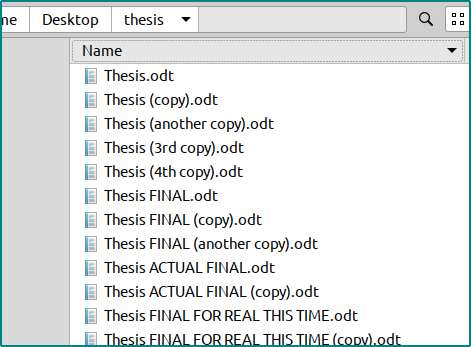
\includegraphics[width=\textwidth]{images/backups.png}%
    \end{column}
  \end{columns}
\end{frame}

\begin{frame}
  \frametitle{Short fact sheet}

  \begin{columns}
    \begin{column}{.72\textwidth}
      \begin{itemize}
        \item Git is a~\alert{Distributed Version Control System}.
        \item Created in 2005 by \alert{Linus Torvalds}\\%
          (the creator of Linux).
        \item Free and Open-Source Software.
        \item Probably the most popular VCS out there.
      \end{itemize}
    \end{column}

    \begin{column}{.28\textwidth}
      {\tiny{}%
        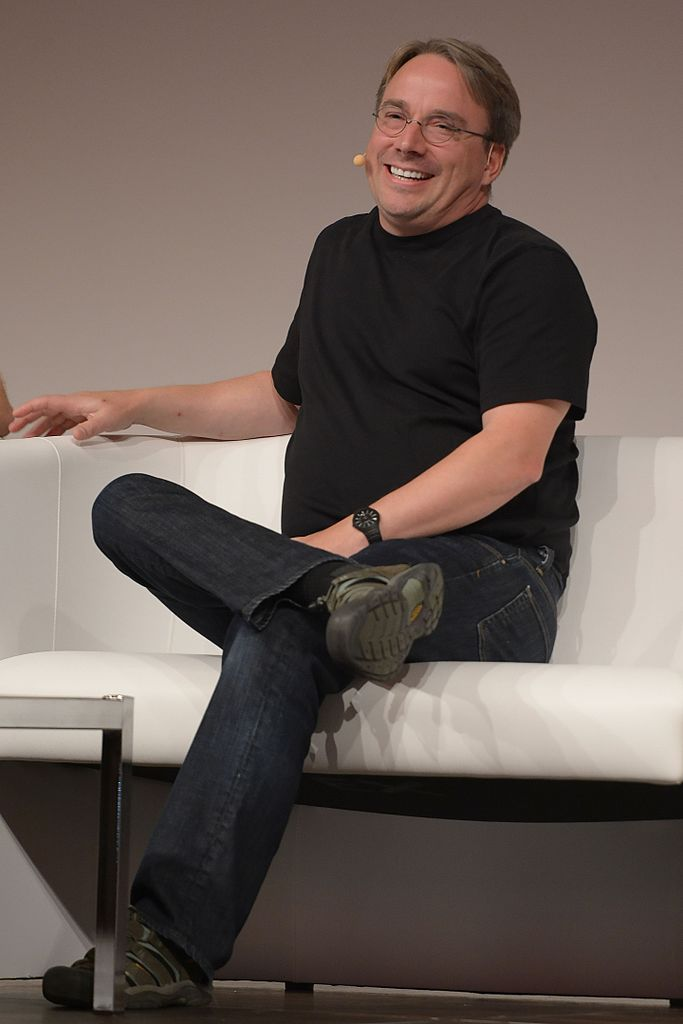
\includegraphics[width=\textwidth]{images/linus-torvalds.jpg}\\%
        Photo: Krd (\href{https://creativecommons.org/licenses/by-sa/3.0}{CC BY-SA 3.0}),
        via Wikimedia Commons%
        \par%
      }
    \end{column}
  \end{columns}
\end{frame}

\begin{frame}
  \frametitle{Version control}

  A~\alert{Version Control System} (VCS) keeps track of different versions of
  a project.
\end{frame}

\begin{frame}
  \frametitle{Two meanings of `version'}

  \begin{block}{Meaning 1}
    `Version' as in the state of a~project at a~given point in time.\\
    $\rightarrow$ i.\,e.\ `old version' vs.\ `new version'
  \end{block}
  \centering{%
    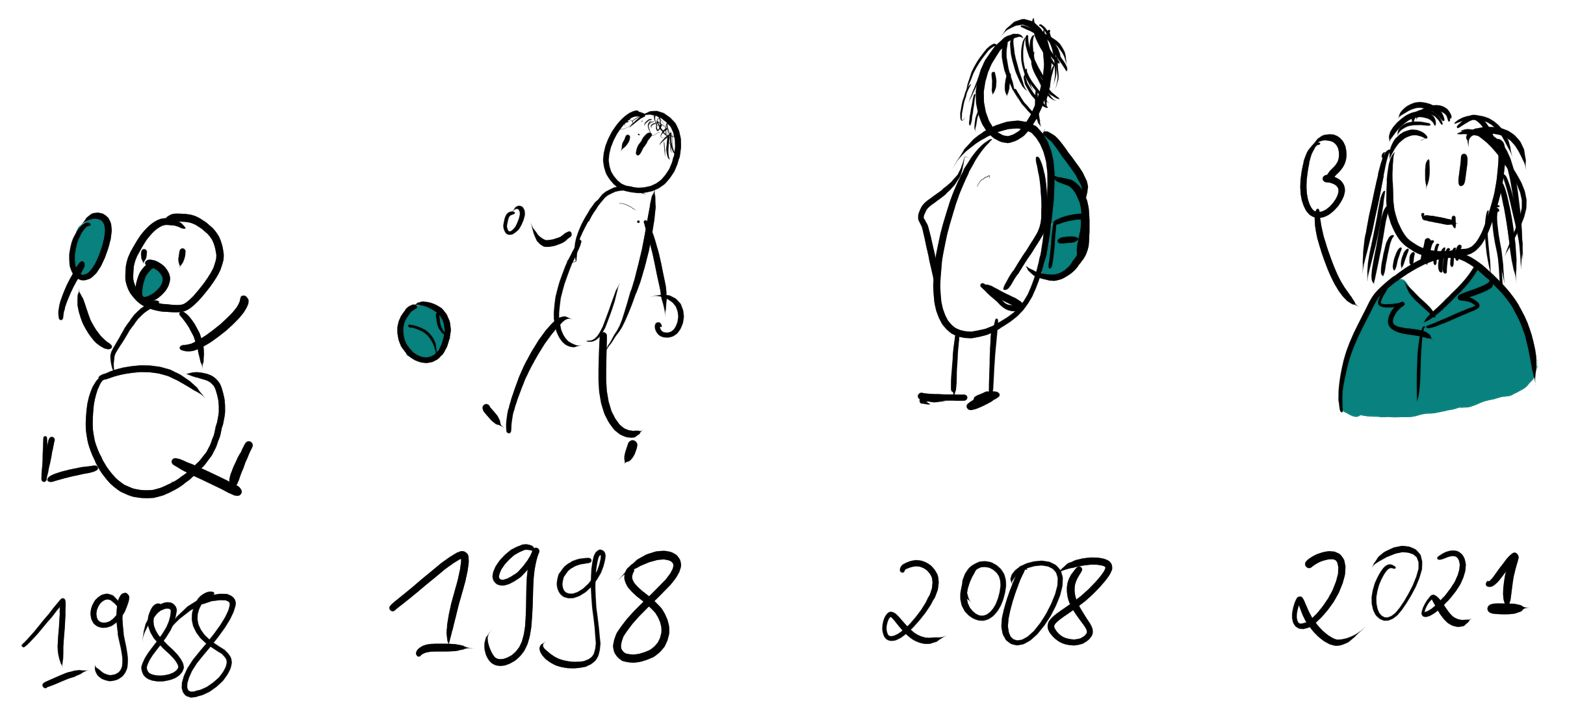
\includegraphics[width=.75\textwidth]{images/versions-over-time.jpg}%
  }
\end{frame}

\begin{frame}
  \frametitle{Two meanings of `version' (ctd.)}

  \begin{block}{Meaning 2}
    `Version' as in different alternative editions of the same project, existing
    next to each other.\\
    $\to$ `regular version' vs.\ `evil alternate universe version'
  \end{block}
  \centering{%
    
\includegraphics[width=.65\textwidth]{images/versions-parallel.jpg}%
  }
\end{frame}

\begin{frame}
  \frametitle{Two meanings of `version' (ctd.)}

  Version Control Systems do both!\\
  \centering{%
    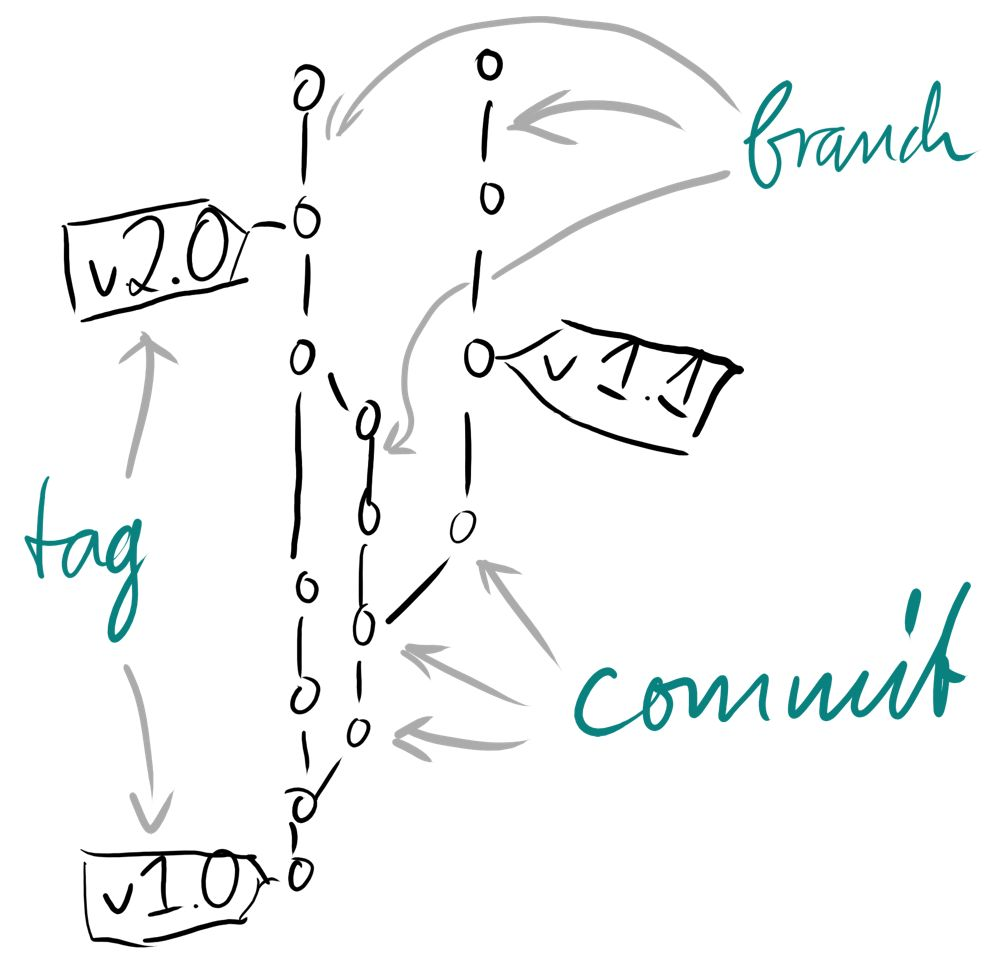
\includegraphics[width=.5\textwidth]{images/terminology.jpg}%
  }
\end{frame}

\begin{frame}
  \frametitle{What can VCS's be used for?}

  \begin{itemize}
    \item Programming
    \item Configuration files
    \item Writing an article together in \LaTeX, Markdown, etc.
    \item \alert{Reproducible and citable research data}\\
      (we like that around here)
    \item Personal to-do lists, notes, etc.
    \item These slides \texttt{;\rparen}
  \end{itemize}
\end{frame}

\begin{frame}
  \frametitle{Know your limits!}

  \begin{block}{What are VCS's good at?}
    Text-based data
    (plain-text files, program code, XML/HTML, \LaTeX, CSV tables, etc.)
  \end{block}

  \begin{block}{What are (most) VCS's bad at?}
    Binary data
    (images, audio files, pdfs, zip archives, etc.)
  \end{block}
\end{frame}

\begin{frame}
  \frametitle{Centralised vs.\ Distributed VCS }

    \centering{%
      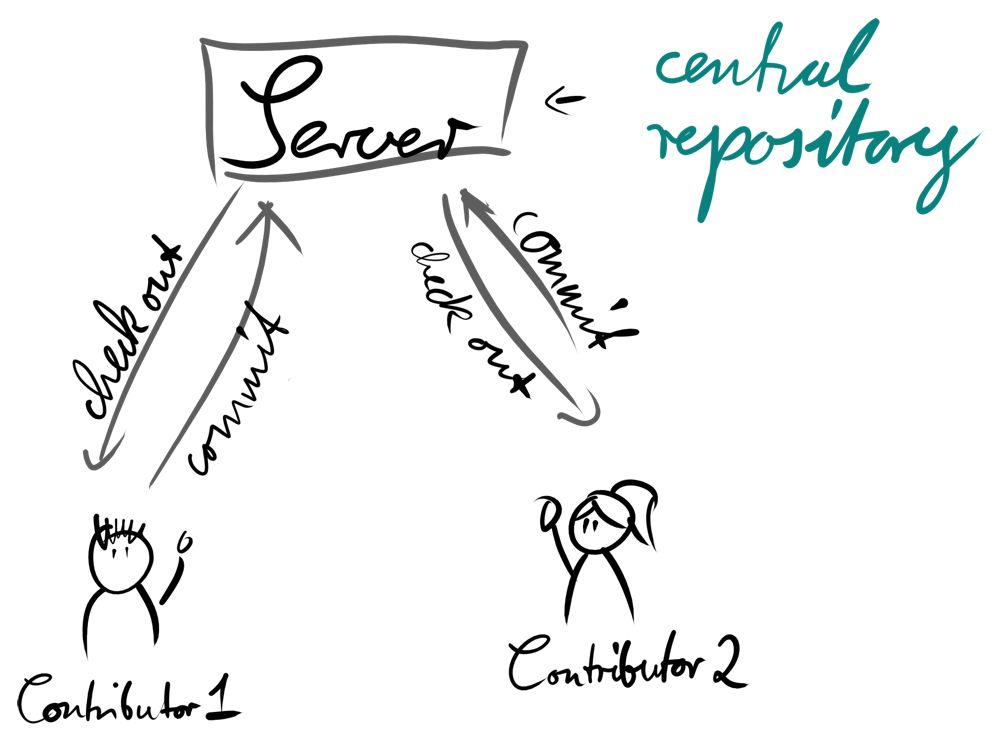
\includegraphics[width=.5\textwidth]{images/centralised-vcs.jpg}%
    }
    \begin{block}{Centralised VCS (e.\,g.\ CVS, subversion)}
      \begin{itemize}
        \item Central repository on some server somewhere.
        \item People download the current state of the project to their computers.
        \item People upload any changes they made back onto the server.
      \end{itemize}
    \end{block}
\end{frame}

\begin{frame}
  \frametitle{Centralised vs.\ Distributed VCS (ctd.)}

  \centering{%
    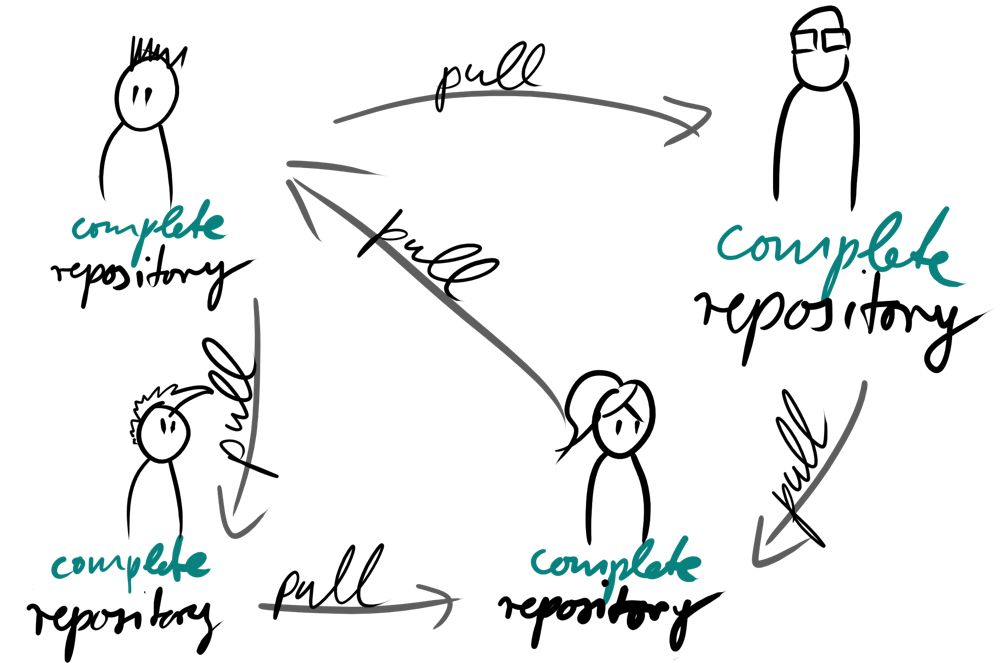
\includegraphics[width=.5\textwidth]{images/distributed-vcs.jpg}%
  }
  \begin{block}{Distributed Version Control (e.\,g.\ git, mercurial)}
    \begin{itemize}
      \item Everybody has a~complete copy of the project (and all its history)
        on their hard drives.
      \item Changes are pushed and pulled between the different repositories.
    \end{itemize}
  \end{block}
\end{frame}

\begin{frame}
  \frametitle{Centralised vs.\ Distributed VCS (ctd.)}

  \begin{block}{Note}
    In reality, people put a~separate copy of the project on a~server somewhere
    and pull/push their changes through that.
    \begin{itemize}
      \item Some project spin up their own git servers, e.\,g.:
        \begin{itemize}
          \item \href{https://git.kernel.org/}{Linux kernel$^{\hookrightarrow}$}
          \item \href{https://savannah.gnu.org/}{GNU operating system$^{\hookrightarrow}$}
        \end{itemize}
      \item Others use third-party hosting sites:
        \begin{itemize}
          \item \href{https://github.com}{Microsoft's Github$^{\hookrightarrow}$}
            (most popular)
          \item \href{https://bitbucket.org}{Atlassian's Bitbucket$^{\hookrightarrow}$}
          \item \href{https://about.gitlab.com}{Gitlab$^{\hookrightarrow}$}
        \end{itemize}
    \end{itemize}
  \end{block}
\end{frame}

\begin{frame}
  \frametitle{Know your limits! (ctd.)}

  \begin{block}{Advantages of Distributed Version Control}
    \begin{itemize}
      \item No need for a~constant internet connection.
      \item Quick and comfy workflow (local branches are the best!).
      \item The massive redundancy reduces the chance of data loss.
    \end{itemize}
  \end{block}

  \begin{block}{Drawbacks}
    \begin{itemize}
      \item Workflow of pulling/merging can be a~bit finicky at times.
      \item Copies get out of sync with each other more easily, increasing the
        number of merge conflicts.
      \item Copying around the entire history wastes disk space and bandwidth,
        and also just takes longer.
    \end{itemize}
  \end{block}
\end{frame}

\begin{frame}
  \frametitle{Quick terminology note}

  \begin{block}{What is a~`repository'?}
    {\footnotesize{}(coll.: \alert{repo} or \alert{repos})}
    \begin{itemize}
      \item General tech speak:
        online storage space
      \item Git speak:
        a~copy of a~version-controlled project folder
    \end{itemize}
  \end{block}
\end{frame}


\section{Getting git set up}

\begin{frame}[fragile]
  \frametitle{Download/Installation}

  \begin{itemize}
    \item GNU/Linux, *BSD: it's in the repos
    \item Windows: \href{https://git-scm.com/downloads}{https:/\kern-.5ex/git-scm.com/downloads}
    \item macOS:
      \begin{itemize}
        \item Option 1: install the XCode command-line tools:\\
          \verb"$ xcode-select --install"
        \item Option 2: \href{https://git-scm.com/downloads}{https:/\kern-.5ex/git-scm.com/downloads}
        \item Option 3: it's on homebrew
      \end{itemize}
  \end{itemize}
\end{frame}

\begin{frame}[fragile]
  \frametitle{User interface}

  \begin{itemize}
    \item Git uses a~command-line interface
    \item There are graphical interfaces and editor plugins for common tasks,
      but at the end of the day the command-line is the preferred way to use git
  \end{itemize}
  {\footnotesize{}%
    \begin{verbatim}
$ git
usage: git [--version] [--help] [-C <path>] [-c <name>=<value>]
           [--exec-path[=<path>]] [--html-path] [--man-path] [--info-path]
           [-p | --paginate | -P | --no-pager] [--no-replace-objects] [--bare]
           [--git-dir=<path>] [--work-tree=<path>] [--namespace=<name>]
           <command> [<args>]

These are common Git commands used in various situations:
[...]
    \end{verbatim}
  }
\end{frame}

\begin{frame}[fragile]
  \frametitle{First setup}

  \begin{block}{Tell git your name and email address}
    {\footnotesize{}%
      \begin{verbatim}
$ git config --global user.name "Johannes Englisch"
$ git config --global user.email "englisch@shh.mpg.de"
      \end{verbatim}%
    }
    \begin{itemize}
      \item The name and address will be attached to \alert{every commit} you
        make.
      \item This is completely unrelated to any
        Github/\hspace{0}Bitbucket/\hspace{0}etc.\ accounts you might have!
    \end{itemize}
  \end{block}
\end{frame}

\begin{frame}[fragile]
  \frametitle{First setup (ctd.)}

  \begin{block}{Tell git about your text editor}
    {\footnotesize{}%
      \begin{verbatim}
$ git config --global core.editor "C:\Program Files\Notepad++\Notepad++.exe"
$ git config --global core.editor "/usr/bin/emacs"
$ ...
      \end{verbatim}%
    }
    $\to$ The official installer also allows to set the editor
    (at least on Windows).
  \end{block}
\end{frame}

\begin{frame}[fragile]
  \frametitle{First setup (ctd.)}

  \begin{block}{Avoid potential headache regarding line endings}
    \begin{itemize}
      \item Windows: \\{}
        {\footnotesize{}\verb"$ git config --global core.autocrlf true"}
      \item GNU/Linux, *BSD, macOS, etc.:\\{}
        {\footnotesize{}\verb"$ git config --global core.autocrlf input"}
    \end{itemize}
  \end{block}
\end{frame}

\begin{frame}[fragile]
  \frametitle{First setup (ctd.)}

  \begin{block}{Review your settings}
    {\footnotesize{}%
      \begin{verbatim}
$ git config -l
      \end{verbatim}%
    }
  \end{block}
\end{frame}

\section{Exploring a git repo}

\begin{frame}[fragile]
  \frametitle{Cloning an existing repo}

  {\footnotesize{}%
    \begin{verbatim}
$ git clone https://github.com/dictionaria/kalamang kalamang
Cloning into 'kalamang'...
remote: Enumerating objects: 155, done.
remote: Counting objects: 100% (155/155), done.
remote: Compressing objects: 100% (81/81), done.
remote: Total 155 (delta 81), reused 139 (delta 68), pack-reused 0
Receiving objects: 100% (155/155), 927.47 KiB | 7.73 MiB/s, done.
Resolving deltas: 100% (81/81), done.
    \end{verbatim}%
  }
\end{frame}

\begin{frame}[fragile]
  \frametitle{Status report!}

  {\footnotesize{}%
    \begin{verbatim}
$ cd kalamang
$ git status
On branch main
Your branch is up-to-date with 'origin/main'.

nothing to commit, working tree clean
    \end{verbatim}%
  }
\end{frame}

\begin{frame}[fragile]
  \frametitle{History lesson}

  {\footnotesize{}%
    \begin{verbatim}
$ git log
commit 5f28ae268e88d70e2f5f9ca2497a7e8fed257611 (HEAD -> main, tag: v1.1, origin/main, origin/HEAD)
Author: Robert Forkel <...>
Date:   Fri Apr 9 13:27:29 2021 +0200

    re-compiled against Glottolog 4.3

commit 3d98441885adb1037afcbde9478d8ae4c0330567
Author: Johannes Englisch <englisch@shh.mpg.de>
Date:   Wed Apr 7 14:41:57 2021 +0200

    regen with current pydictionaria version
[...]
    \end{verbatim}%
  }
\end{frame}

\begin{frame}[fragile]
  \frametitle{Branches, Tags}

  {\footnotesize{}%
    \begin{verbatim}
$ git branch
* main
$ git branch -a
* main
  remotes/origin/HEAD -> origin/main
  remotes/origin/link-to-concepticon
  remotes/origin/main
$ git tag
v1.0
v1.1
    \end{verbatim}%
  }
\end{frame}

\begin{frame}[fragile]
  \frametitle{Time to time travel}

  {\footnotesize{}%
    \begin{verbatim}
$ git checkout v1.0
[...]
HEAD is now at 64ba30e release 1.0
$ git checkout link-to-concepticon
[...]
Switched to a new branch 'link-to-concepticon'
$ git checkout d1e45b9
[...]
HEAD is now at d1e45b9 metadata regen
    \end{verbatim}
  }
  $\to$ re.\ commits: you don't have to type all 40 digits -- only enough
  to make it unique (usually like 7 or so digits)
\end{frame}


\section{Your very own git repo}

\begin{frame}[fragile]
  \frametitle{Creating a~new git repo}

  {\footnotesize{}%
    \begin{verbatim}
$ cd <folder>
$ git init
Initialised empty Git repository in <folder>/.git
    \end{verbatim}%
  }
\end{frame}

\begin{frame}[fragile]
  \frametitle{Reviewing your changes}

  \begin{block}{What files changed since the last commit?}
    {\footnotesize{}%
      \begin{verbatim}
$ git status
      \end{verbatim}%
    }
  \end{block}

  \begin{block}{What lines changed since the last commit?}
    {\footnotesize{}%
      \begin{verbatim}
$ git diff
      \end{verbatim}%
    }
  \end{block}
\end{frame}

\begin{frame}
  \frametitle{Making a~commit is a two-step process}

  \centering{%
    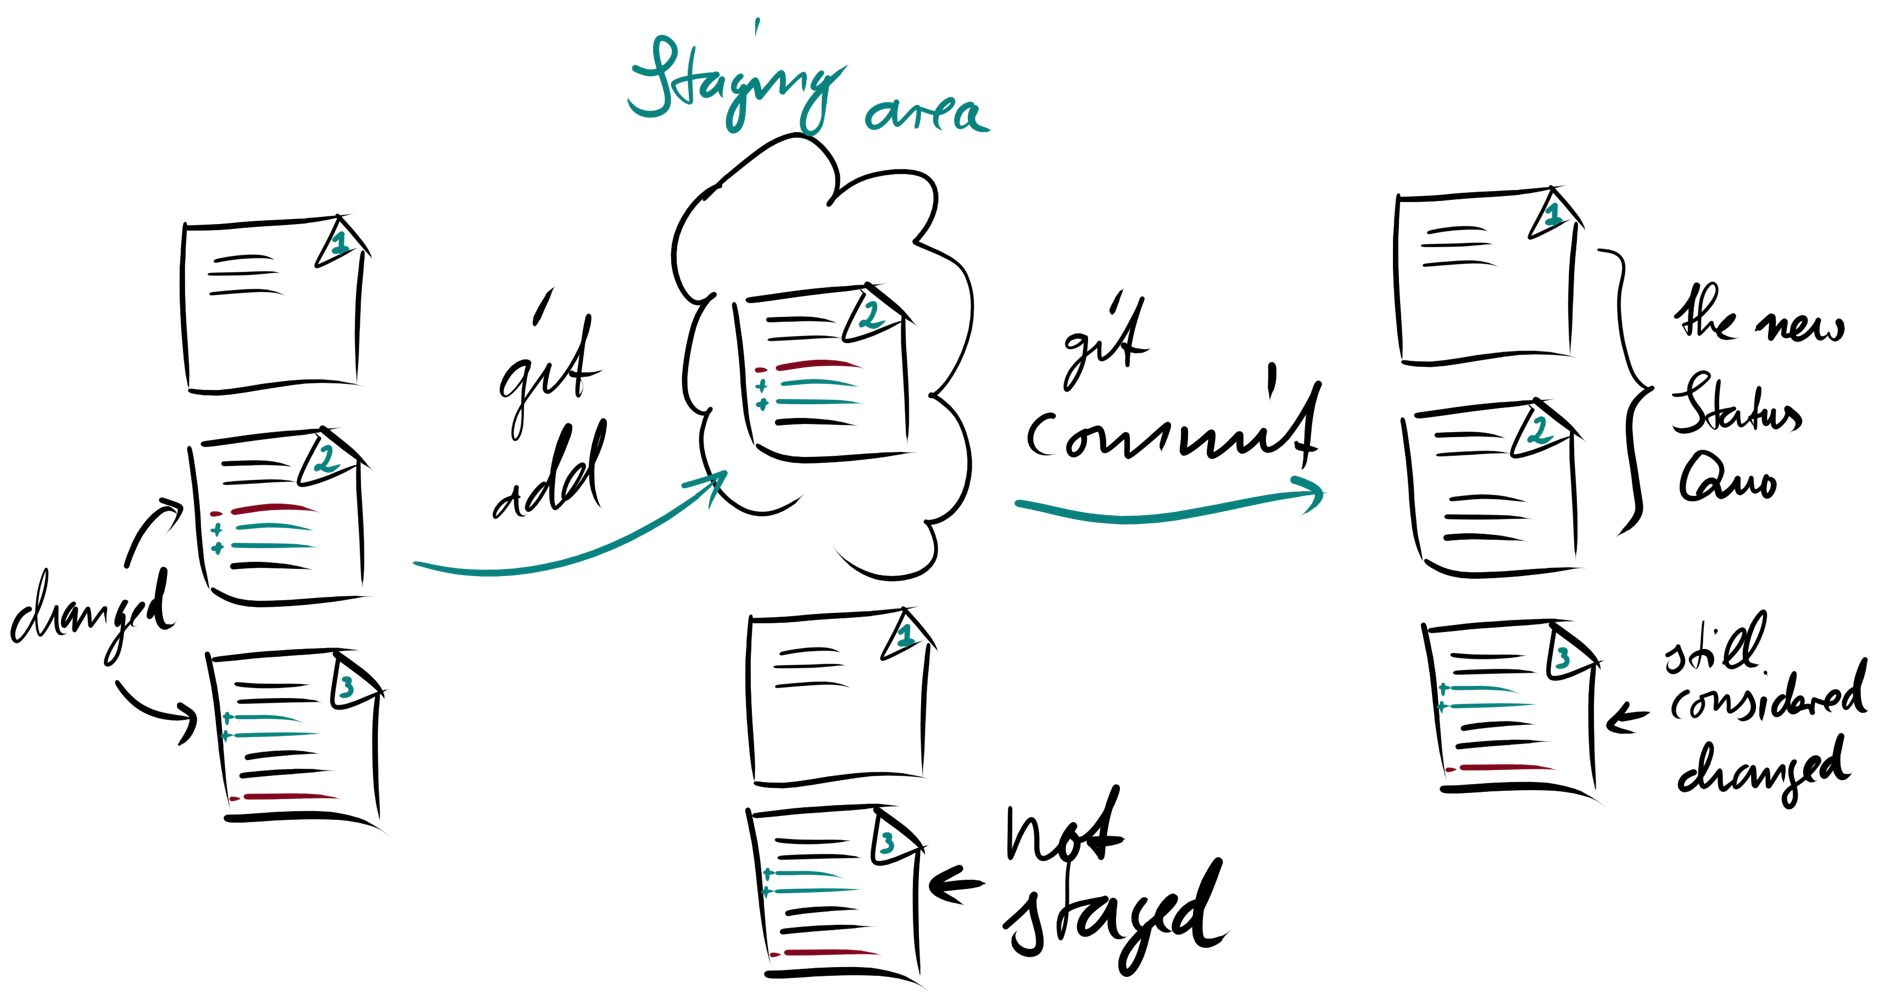
\includegraphics[width=.9\textwidth]{images/staging.jpg}%
  }
  \begin{enumerate}
    \item\alert{Add} changes to the Staging Area.
    \item\alert{Commit} to these changes (and leave a~commit message).
  \end{enumerate}
\end{frame}

\begin{frame}[fragile]
  \frametitle{Adding changes to the staging area}

  {\footnotesize{}%
    \begin{verbatim}
$ git add file1 file2 [...]
    \end{verbatim}%
  }
\end{frame}

\begin{frame}[fragile]
  \frametitle{Time for some commitment}

  \begin{block}{Short version}
    {\footnotesize{}%
      \begin{verbatim}
$ git commit -m "short, yet helpful commit message :D"
      \end{verbatim}%
    }
  \end{block}

  \begin{block}{`Proper' version}
    {\footnotesize{}%
      \begin{verbatim}
$ git commit
      \end{verbatim}%
    }
  \end{block}

  The latter will open your text editor for your commit message:
  \begin{itemize}
    \item Save$+$quit to create the commit.
    \item Leave the message blank (or quit without saving) to abort the commit.
  \end{itemize}
\end{frame}

\begin{frame}
  \frametitle{Good and helpful commit messages}

  \centering{\tiny{}%
    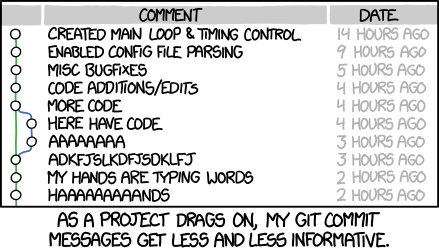
\includegraphics[width=.5\textwidth]{images/xkcd-git-commit.png}\\%
    by Randall Monroe
    (\href{https://creativecommons.org/licenses/by-nc/2.5/}{CC BY-NC 2.5}),
    \href{https://xkcd.com/1296/}{https:/\kern-.5ex/xkcd.com/1296/}%
    \par%
  }
\end{frame}

\begin{frame}
  \frametitle{Good and helpful commit messages (ctd.)}

  \centering{%
    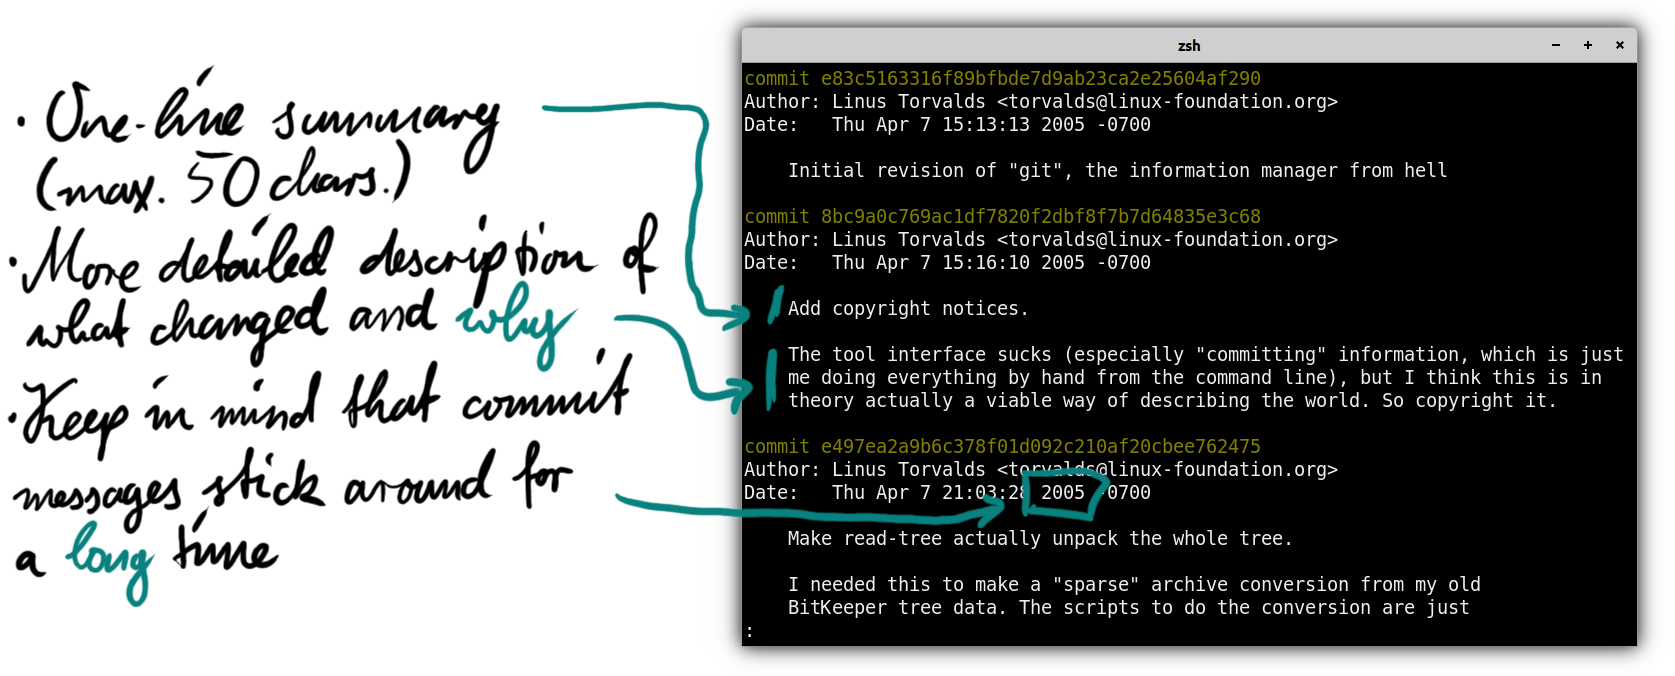
\includegraphics[width=\textwidth]{images/good-commit-message.png}%
  }
\end{frame}

\begin{frame}
  \frametitle{Good and helpful commit messages (ctd.)}

  \begin{block}{Good one-liners}
    A~good technique for a~one-line commit message is to focus more on
    \alert{why} a~commit was made.\\
  \end{block}

  \begin{block}{Example}
    \begin{tabular}{@{}ll@{}}
      don't: & \sout{\texttt{updated readme}} \\
      do:    & \texttt{forgot Steve in the author listing} \\
    \end{tabular}
  \end{block}
\end{frame}

\begin{frame}[fragile]
  \frametitle{Changing your mind}

  \begin{block}{I'm not ready to commit to this yet!}
    {\footnotesize{}%
      \begin{verbatim}
$ git reset file.txt
      \end{verbatim}%
    }
    Note: This does \alert{not delete or change} any files -- it just removes
    them from the Staging Area.
  \end{block}
\end{frame}

\begin{frame}[fragile]
  \frametitle{Changing your mind (ctd.)}

  \begin{block}%
    {%
      Crap, I~messed around with the project and now everything is terrible!
      Let's just throw this away and start over\dots{}%
    }
    {\footnotesize{}%
      \begin{verbatim}
$ git checkout file.txt
      \end{verbatim}%
    }
    \begin{itemize}
      \item This will undo any changes to \texttt{file.txt} that haven't been
        \alert{committed or staged}, yet.
      \item This process is \alert{irreversible} -- tread with caution!
      \item Yes, \texttt{checkout} serves double-duty\dots{}
    \end{itemize}
  \end{block}
\end{frame}

\begin{frame}[fragile]
  \frametitle{Ignore me}

  \begin{block}
    {%
      There are a~bunch of (temp) files in my folder that I~don't want to add to
      my git repo%
    }
    \begin{itemize}
      \item Create a~text file called \texttt{.gitignore}\\%
        (nothing before the dot; no extension at the end).
      \item Add a~new line for every file you want to ignore.
      \item The \texttt{.gitignore} file is just another file you can
        add/\hspace{0}commit/\hspace{0}etc.\ to your git repo.
    \end{itemize}
  \end{block}
\end{frame}

% adding a tag?


\section{Publish your work on Github}

\begin{frame}
  \frametitle{Basic idea}

  \begin{itemize}
    \item Create an empty git repo on Github (or anywhere else).
    \item Tell your local git repo about it.
    \item Push your local history to the remote repo.
  \end{itemize}
\end{frame}

\begin{frame}
  \frametitle{Alternative workflow for new projects}

  \begin{itemize}
    \item Create an empty git repo on Github (or anywhere else).
    \item Clone the empty onto your computer.
  \end{itemize}
\end{frame}

\begin{frame}
  \frametitle{Github does not know who you are}

  \begin{itemize}
    \item You can only clone/pull from repos you have read access to.
    \item You can only push to repos you have write access to.
    \item Git needs to send some sort of ID or else Github will refuse to
      cooperate.
    \item Git cannot look into your browser, so being logged on to the Github
      website doesn't do anything\dots{}
  \end{itemize}
\end{frame}

\begin{frame}
  \frametitle{Two methods}

  \begin{itemize}
    \item Personal access token\\
      (not gonna cover that one here -- check
      \href{https://docs.github.com/en/github/authenticating-to-github/keeping-your-account-and-data-secure/creating-a-personal-access-token#creating-a-token}%
      {Github's documentation$^{\hookrightarrow}$} for details)
    \item Secure Shell (SSH)
  \end{itemize}
\end{frame}

\begin{frame}[fragile]
  \frametitle{Secure Shell (SSH)}

  \begin{block}{Create a~key pair (if you don't have one yet)}
    {\footnotesize{}%
      \begin{verbatim}
$ ssh-keygen -t ed25519 -C "your_email@example.com"
      \end{verbatim}
    }
  \end{block}

\end{frame}

\begin{frame}
  \frametitle{Secure Shell (ctd.)}

  \begin{block}{Find your public key}
    \centering{%
      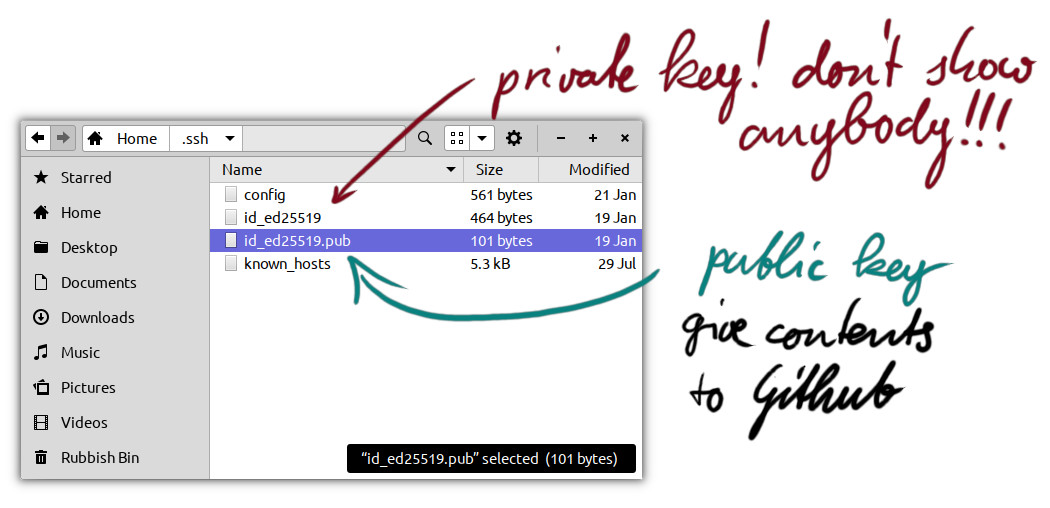
\includegraphics[width=.9\textwidth]{images/ssh-keys.jpg}%
    }
  \end{block}
\end{frame}

\begin{frame}
  \frametitle{Secure Shell (ctd.)}

  \begin{block}{Give your public key to Github}
    \centering{%
      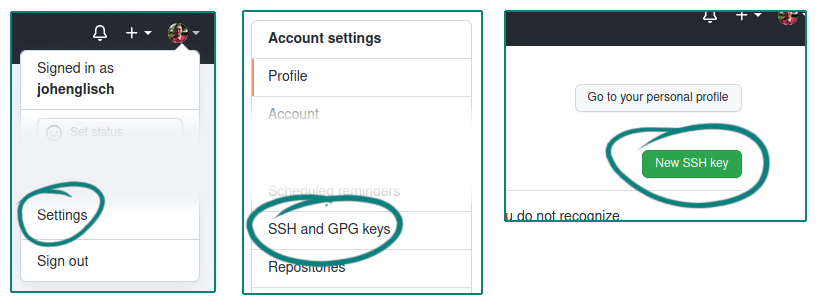
\includegraphics[width=.75\textwidth]{images/add-ssh-key.png}%
    }
  \end{block}
\end{frame}

\begin{frame}
  \frametitle{Creating a~new repo on Github}

  \centering{%
    
\includegraphics[width=.5\textwidth]{images/new-repo.png}%
  }
\end{frame}

\begin{frame}[fragile]
  \frametitle{Cloning a~git repo over SSH}

  \begin{itemize}
    \item Cloning over SSH requires a~different URL than regular cloning:\\
      {\footnotesize{}\verb"git@github.com:<user name>/<repo name>"}
  \end{itemize}
  {\footnotesize{}%
    \begin{verbatim}
$ git clone git@github.com:johenglisch/2021-git-intro
    \end{verbatim}%
  }
\end{frame}

% register ssh key on github?
% make slide repo
% setup remote + pull
% push

% clone a separate version as proof

% add + commit
% push

% fetch + merge

\end{document}
